\documentclass[tikz,border=4pt]{standalone}
\usepackage{amsmath,amssymb}

\usetikzlibrary{arrows.meta,positioning,automata,shapes,shapes.misc,calc,decorations.pathmorphing,decorations.markings,angles,quotes,patterns,mindmap,matrix,knots,hobby,trees}
\tikzset{->-/.style={decoration={markings, mark=at position 0.5 with {\arrow{Stealth}}}, postaction={decorate}}}
\begin{document}
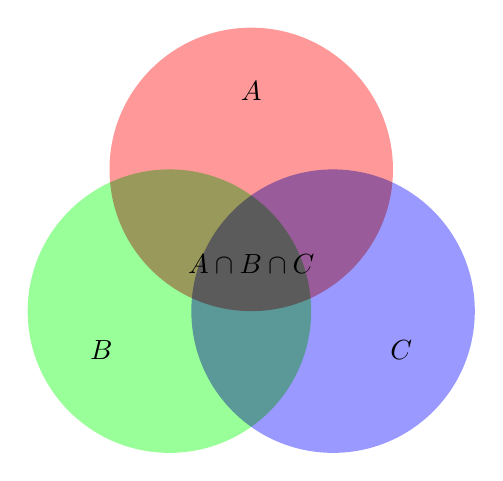
\begin{tikzpicture}
\begin{scope}[blend group=multiply]
\fill[red!40] (90:1.2) circle (1.8); \fill[green!40] (210:1.2) circle (1.8); \fill[blue!40] (330:1.2) circle (1.8);
\end{scope}
\node at (90:2.2) {$A$}; \node at (210:2.2) {$B$}; \node at (330:2.2) {$C$}; \node {$A\cap B\cap C$};
\end{tikzpicture}
\end{document}
